% !TEX root = Thesis.tex

%==============================================================================
\chapter{Results and discussion}
\label{chap:results_and_discussion}
%==============================================================================

Once the theoretical description of the experiment has been completely introduced, the following part consist in the exposition of the obtained results together with a discussion concerning its correspondence with the announced theory. Due to this, the first step must be the Raman beams characterization with the measurement of each beam radius. This will allow in the next parts to make a direct correlation between beam power and intensity, which will be crucial for the whole experiment characterization.

\section{Measurement of the Raman beams radius}

These laser beams of the \SI{841}{\nano\meter} transition have been considered during all the theory as Gaussian beams. Therefore, they are described spatially by Equation \eqref{eq:intensity_gaussian}, which gives the relation between beam power $P$ and maximum intensity $I_{0}$ as
\begin{equation}
	I_0 = \frac{2P}{\pi w_0^2}
\end{equation}

Where $w_0$ represents the beam radius at the atomic cloud position. Thus, a measurement of this quantity must be performed in order to obtain $I_0$ from the beam power. Figure \ref{fig:raman_beams_radius} shows both horizontal and vertical measurements for the two beams with the use of a knife-edge method. These data points were fit to an error function, which gave the estimations for $w_0$ in every case. From averaging the vertical and horizontal estimations of $w_0$ one gets the final measurement to be
\begin{align*}
	w_{01} &= (0.4961\pm0.0012)\si{\milli\meter}   &   w_{02} &= (0.8778\pm0.0024)\si{\milli\meter}
\end{align*}

Note that the use of 1 and 2 for the Raman beams is also used as a distinction tool in Figure \ref{fig:raman_set_up}. As one can observe, the difference in size between both beams is approximately a factor of 3. This must be compensated by adjusting the beam powers; however, it is a strong mismatch in the parameters that could not be solved due to time constraints. Therefore, the discussion part of the following measurements will have into account this mismatch in beam sizes as a source of possible non-correspondence between theory and experiment.

\pagebreak

\begin{figure}
	\centering
	\begin{subfigure}{.5\textwidth}
		\centering
		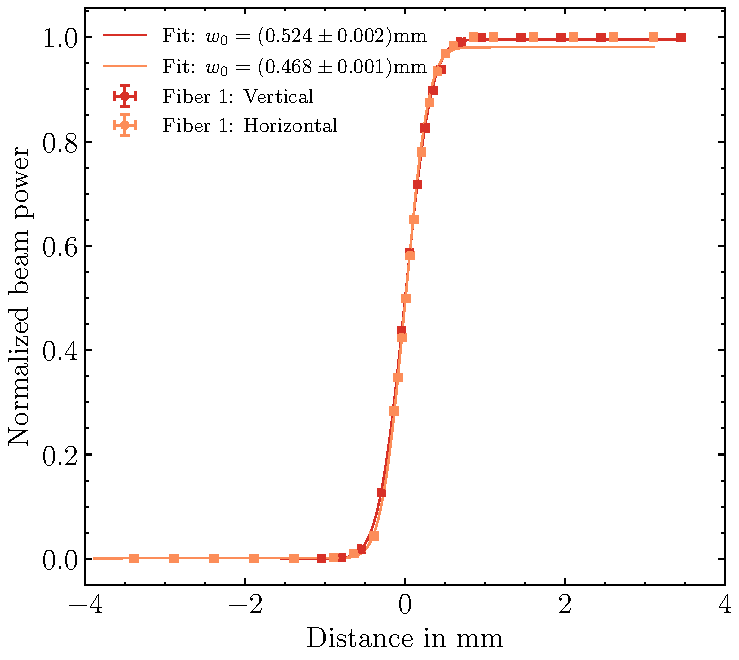
\includegraphics[width=1.\linewidth]{Fiber 1.pdf}
		\caption{Raman beam 1 (R1)}
		\label{fig:raman_beams_radius_1}
	\end{subfigure}%
	\begin{subfigure}{.5\textwidth}
		\centering
		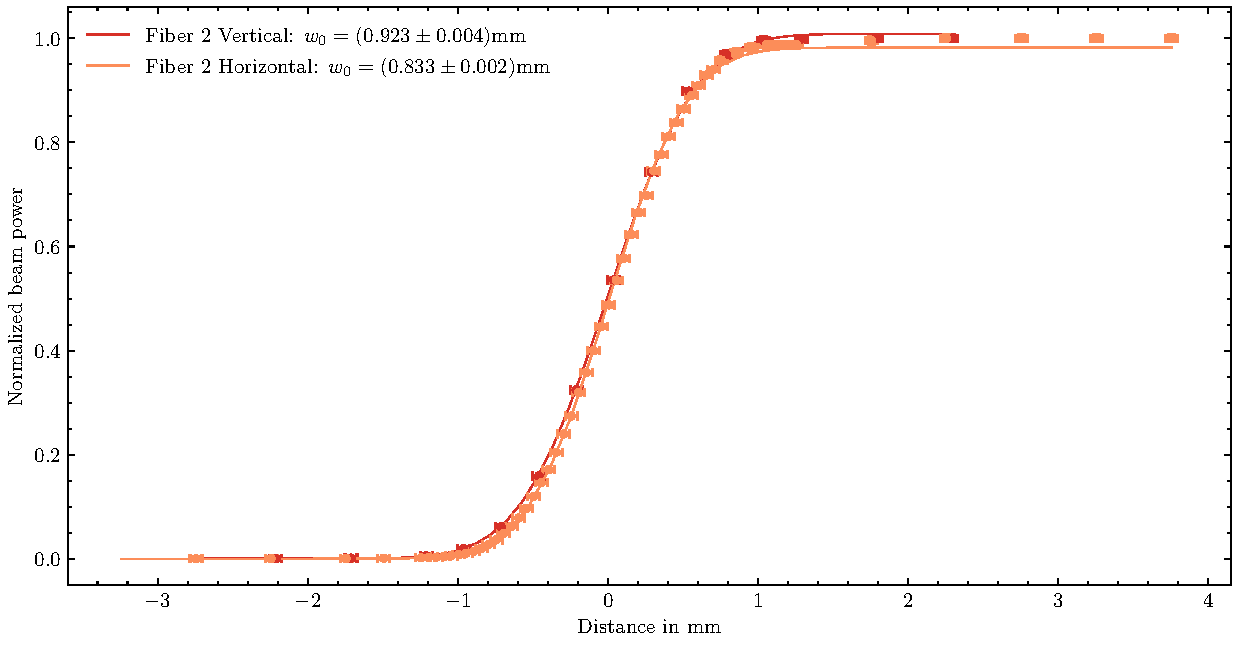
\includegraphics[width=0.955\linewidth]{Fiber 2.pdf}
		\caption{Raman beam 2 (R2)}
		\label{fig:raman_beams_radius_2}
	\end{subfigure}
	\caption[Beam radius measurement of the Raman beams performed with a knife-edge method]{Beam radius measurement of the Raman beams performed with a knife-edge method. The beam profile was measured at approximately the atomic cloud position. Each of the beams were measured in a vertical (red) and horizontal (orange) position.}
	\label{fig:raman_beams_radius}
\end{figure}


\section{Spectroscopy of the \SI{841}{\nano\meter} erbium transition with a \ac{bec}}

%%% Local Variables: 
%%% mode: latex
%%% TeX-master: "Thesis"
%%% End: 
